	\documentclass[10pt]{article}
	\usepackage[top=1.5cm, bottom=1.5cm, left=1.5cm, right=1.5cm]{geometry}
	\usepackage{lineno}
	\usepackage{fontspec}
	\usepackage{graphicx}
	\usepackage{textcomp}
	\usepackage{blindtext}
	\usepackage[utf8]{inputenc}
	\usepackage{eurosym}
	\usepackage{titlesec}
	\usepackage[bottom]{footmisc}
	\usepackage{array}
	\usepackage{enumitem}
	\usepackage{hyperref}
	\usepackage{color}
	\usepackage{framed}
	\usepackage{amsmath}
	\usepackage{float}
	\usepackage{amssymb}
	\usepackage{listings}	
	\definecolor{dkgreen}{rgb}{0,0.6,0}
	\definecolor{ltgray}{rgb}{0.5,0.5,0.5}
	\lstset{
  	backgroundcolor=\color{white},
  	basicstyle=\footnotesize,
  	breakatwhitespace=false,
  	breaklines=true,
  	captionpos=b,
  	commentstyle=\color{dkgreen},
  	deletekeywords={...},
  	escapeinside={\%*}{*)},
  	extendedchars=true,
  	frame=single,
  	keepspaces=true,
  	keywordstyle=\color{blue},
  	language=SQL,
  	morekeywords={*,modify,MODIFY,..., DELIMITER},
  	numbers=left,
  	numbersep=15pt,
  	numberstyle=\tiny,
  	rulecolor=\color{ltgray},
  	showspaces=false,
  	showstringspaces=false, 
  	showtabs=false,
  	stepnumber=1,
  	tabsize=4,
  	title=\lstname
}
	%\ Creazione nuova indentazione "subsubsubsection" 
	\titleclass{\subsubsubsection}{straight}[\subsection]
	
	\newcounter{subsubsubsection}[subsubsection]
	\renewcommand\thesubsubsubsection{\thesubsubsection.\arabic{subsubsubsection}}
	\renewcommand\theparagraph{\thesubsubsubsection.\arabic{paragraph}} % optional; useful if paragraphs are to be numbered
	
	\titleformat{\subsubsubsection}
	  {\normalfont\normalsize\bfseries}{\thesubsubsubsection}{1em}{}
	\titlespacing*{\subsubsubsection}
	{0pt}{3.25ex plus 1ex minus .2ex}{1.5ex plus .2ex}
	
	\makeatletter
	\renewcommand\paragraph{\@startsection{paragraph}{5}{\z@}%
	  {3.25ex \@plus1ex \@minus.2ex}%
	  {-1em}%
	  {\normalfont\normalsize\bfseries}}
	\renewcommand\subparagraph{\@startsection{subparagraph}{6}{\parindent}%
	  {3.25ex \@plus1ex \@minus .2ex}%
	  {-1em}%
	  {\normalfont\normalsize\bfseries}}
	\def\toclevel@subsubsubsection{4}
	\def\toclevel@paragraph{5}
	\def\toclevel@paragraph{6}
	\def\l@subsubsubsection{\@dottedtocline{4}{7em}{4em}}
	\def\l@paragraph{\@dottedtocline{5}{10em}{5em}}
	\def\l@subparagraph{\@dottedtocline{6}{14em}{6em}}
	\makeatother
	
	\setcounter{secnumdepth}{4}
	\setcounter{tocdepth}{4}
	
	\makeindex
	\setmainfont{Arial}
	\usepackage[english, italian]{babel}
	\title{\begin{Huge}Just Eat\end{Huge}}
	\author{Davide Zilio\\Francesco Magarotto\\Written in \LaTeX}
	\date{21 Novembre 2017}
	\renewcommand\thelinenumber{\large\Roman{linenumber}}
	\begin{document}
	\maketitle
	\begin{large}
		\begin{center}
			\LARGE Abstract
		\end{center}
	\begin{linenumbers}
	Just Eat \`e un servizio per la spedizione pasti fondato nel 2005 da Jesper Buch in Regno Unito. Il sito permette al cliente di ordinare comodamente le pietanze da lui preferite e farsele recapitare ovunque lui voglia: al lavoro o a casa. 
	Oggigiorno, l'azienda \`e presente in 13 paesi diversi, e a partire dal 2011 il servizio \`e  attivo anche in Italia. Just Eat propone diversi tipi di cucine a seconda della citt\`a in cui si trova il cliente, e delle attivit\`a ristorative nelle vicinanze con cui la societ\`a inglese ha stretto una partnership. Ad esempio, nella citt\`a di Padova \`e possibile spaziare da un men\`u classico, come la pizza, fino all'innovativa cucina Asianfusion. Il servizio \`e in continua espansione, elaborando migliaia di ordini al mese, e cerca di essere alla portata di tutti: permette ordinazioni telefoniche e pagamento alla consegna, consentendo cos\`i l'utilizzo dei servizio anche a coloro che non sono ``nativi digitali". A quest'ultimi, invece, viene messa a disposizione una pratica applicazione, disponibile per le piattaforme Android\texttrademark{} e iOS\texttrademark{}.
	\end{linenumbers}
	\end{large}
	\pagebreak
	\selectlanguage{italian}
	\tableofcontents{}
	\pagebreak
	\section{Analisi dei requisiti}
	Si vuole realizzare una base di dati che contenga e gestisca gli ordini Just Eat\texttrademark{}, effettuati dai clienti presso i vari ristoranti localizzati nelle diverse citt\`a, individuate tramite il CAP. In particolare, per quanto riguarda i clienti \`e fondamentale che questi siano registrati sul sistema per permettere loro di lasciare un \textit{feedback}, cio\`e un commento relativo alla qualit\`a delle pietanze ricevute, ed effettuare gli ordini presso i vari ristoranti. Quest'ultimi si servono di fattorini\footnotemark{} dipendenti di Just Eat\texttrademark{} che una volta consegnato l'ordine ricevono un punteggio (per ogni ordine completato correttamente, cio\`e completato senza danneggiamenti dovuti al trasporto, l'impiegato riceve un punto in più. In caso contrario, i danneggiamenti vengono segnalati, specificandone la natura, direttamente dall'utente attraverso l'apertura di un \textit{ticket}. Ogni mese il fattorino più giovane con il punteggio più alto riceve un incremento stipendiale di 0,20 \euro{} all'ora. \`E quindi necessario tener conto dei dati anagrafici del fattorino (nome, cognome, codice fiscale, recapito telefonico) e del suo \textbf{stipendio} (composto dalle ore lavorate mensilmente e dallo stipendio all'ora). I clienti sono identificati all'interno della piattaforma attraverso l'indirizzo email che dev'essere confermato, se la conferma non dovesse avvenire, l'utente non può effettuare ordini. Inoltre, per i clienti si ritiene opportuno memorizzare i dati anagrafici come data di nascita, nome, cognome, indirizzo, citt\`a di residenza ed eventuali allergie. I ristoranti mettono a disposizione del cliente un men\`u composto da diverse \textit{pietanze} caratterizzate da un codice univoco, una descrizione, la disponibilit\`a e il costo; la pietanza può essere vegetariana o di altre tipologie, per quanto riguarda le prime si vuole sapere il \textit{metodo di cottura} (al vapore, sottovuoto, al forno). Il cliente nel proprio ordine indica per ogni pietanza desiderata la quantit\`a (espressa in porzioni) di cui necessita, e il metodo di pagamento preferito. Ogni ordine \`e indentificabile in tutta la piattaforma Just Eat\texttrademark{} tramite un codice univoco e contiene l'orario di ricezione dell'ordine e l'orario indicativo di consegna. Per i ristoranti \`e d'interesse sapere la partita iva, il nome, la locazione, il genere culinario, il titolare, un eventuale sito web e il numero di telefono.
	\footnotetext{Si analizza un contesto internazionale dove i fattorini sono dipendenti Just Eat\texttrademark{}. In Italia invece il 90\% di questi sono dipendenti del ristorante dove lavorano}
		\subsection{Glossario dei termini}
		\begin{table}[ht]
		\resizebox{\textwidth}{!}{
			\begin{tabular}{|c|m{6.3cm}|m{5.3cm}|c|}
			 \hline
			  \multicolumn{1}{|c|}{Termine} & \multicolumn{1}{|c|}{Descrizione}&  \multicolumn{1}{|c|}{Attributi}&  \multicolumn{1}{|c|}{Identificatore}\\
			 \hline
			 Cliente& Persona fisica che attraverso telefono o applicazione web ordina pietanze. & Nome, Cognome, CF, Indirizzo, Email, Allergia&   CF \\
			 \hline
			 Ordine&   Ordine eseguito da un cliente.  & Codice, Ora ordinazione, metodo di pagamento   &Codice\\
			 \hline
			 Fattorino& Persona fisica che consegna l'ordine a casa di un cliente. & Nome, Cognome, CF, Data di nascita, Telefono, Stipendio &  CF\\
			 \hline
			 Ristorante& Attivit\`a imprenditoriale munita di partita iva  & Nome, Partita IVA, genere culinario, titolare, indirizzo, sito web e numero di telefono &  Partita iva\\
			 \hline
			 Citt\`a&   Luogo di appartenenza del ristorante e citt\`a di residenza del cliente  & CAP, Nome, Nazione& CAP\\
			 \hline
			 Ticket& Ticket virtuale aperto dal cliente per segnalare a JustEat una problematica relativa alla consegna. & Codice, descrizione & Codice \\
			 \hline 
			 Pietanza & Pietanza realizzata da un ristorante & Codice, nome, prezzo, disponibilit\`a, Descrizione & Codice \\ 
			 \hline
			\end{tabular}
			}
		\end{table}
	\pagebreak
	\section{Progettazione concettuale}
		\subsection{Descrizione testuale delle classi}
			\subsubsection{Citt\`a}
				La classe citt\`a rappresenta la citt\`a e la nazione del ristorante.
				\paragraph{Attributi}
				\begin{itemize}
					\item CAP: \textit{intero $\ll$PK$\gg$} - codice identificativo della citt\`a 
					\item Nome: \textit{stringa} - nome della citt\`a.
					\item Nazione: \textit{stringa} - nazione della citt\`a.
				\end{itemize}
			\subsubsection{Cliente}
				La classe cliente contiene tutte le informazioni di un cliente.
				\paragraph{Attributi}
				\begin{itemize}
					\item CF: \textit{stringa  $\ll$PK$\gg$} - codice fiscale del cliente.
					\item Nome: \textit{stringa} - nome del cliente.
					\item Cognome: \textit{stringa} - cognome del cliente.
					\item Indirizzo: \textit{stringa} - indirizzo di casa del cliente.
				\end{itemize}
				\subsubsubsection{Cliente registrato}
					La classe cliente registrato contiene l'email del cliente registrato a JustEat, la data di attivazione dell'account e le sue eventuali allergie.
				\paragraph{Attributi}
					\begin{itemize}
							\item Email: \textit{stringa  $\ll$PK$\gg$} - email con la quale il cliente si \`e registrato.
							\item Data attivazione: \textit{date} - data di attivazione dell'account del cliente.
							\item Allergia: \textit{stringa} - possibili allergie di un cliente (attributo multivalore 0:N).
					\end{itemize}
			\subsubsection{Ristorante}
				La classe ristorante contiene le informazioni di un ristorante.
				\paragraph{Attributi}
					\begin{itemize}
						\item PIVA: \textit{stringa  $\ll$PK$\gg$} - partita iva del ristorante.
						\item Nome: \textit{stringa}  - nome del ristorante.
						\item Titolare: \textit{stringa} - nome del titotare del ristorante.
						\item Indirizzo: \textit{stringa} - indirizzo del ristorante.
						\item Sito web: \textit{stringa} - sito web del ristorante.
						\item Telefono: \textit{stringa} - recapito telefonico ristorante.
						\item Genere culinario: \textit{stringa} - genere di cucina realizzata nel ristorante.
					\end{itemize}
			\subsubsection{Pietanza}
				La classe pietanza rappresenta il cibo che il ristorante propone e che il cliente registrato ordina.
				\paragraph{Attributi}
					\begin{itemize}
						\item Codice: \textit{stringa  $\ll$PK$\gg$} - codice identificativo della pietanza.
						\item Nome: \textit{stringa} - nome della pietanza.
						\item Descrizione: \textit{string} - descrizione della pietanza.
						\item Costo: \textit{intero} - costo della pietanza.
						\item Disponibilit\`a: \textit{booleano} - presenza o meno della pietanza.
					\end{itemize}
					La pietanza può essere di 2 tipi:
					\begin{itemize}
						\item Altre: pietanze non vegetariane.
						\item Vegetariana: verdura, legumi, [...].
					\end{itemize}
			\subsubsection{Fattorino}
				La classe fattorino contiene le informazioni del fattorino e il suo codice identificativo.
				\paragraph{Attributi}
					\begin{itemize}
						\item CF: \textit{stringa  $\ll$PK$\gg$} - codice fiscale della fattorino.
						\item Nome: \textit{stringa} - nome del fattorino.
						\item Cognome: \textit{stringa} - cognome del fattorino.
						\item Numero di telefono: \textit{intero} - numero telefonico del fattorino.
						\item Stipendio: \textit{stringa} - stipendio del fattorino (ore lavorate + stipendio all'ora).
					\end{itemize}
			\subsubsection{Ordine}
				La classe ordine \`e composta da un codice identificativo e dall'ora in cui l'ordine \`e stato effettuato.
				\paragraph{Attributi}
					\begin{itemize}
						\item Codice: \textit{stringa  $\ll$PK$\gg$} - codice dell'ordinazione.
						\item Orario ordine: \textit{time} - ora dell'ordinazione.
						\item Orario consegna: \textit{time} - ora della consegna dell'ordine.
					\end{itemize}
			\subsubsection{Ticket}
				La classe ticket \`e identificata da un codice e contiene il commento relativo al danneggiamento della pietanza ordinata.
				\paragraph{Attributi}
					\begin{itemize}
						\item Codice: \textit{stringa  $\ll$PK$\gg$} - codice del ticket.
						\item Commento: \textit{stringa} - commento relativo al ticket.
					\end{itemize}
		\subsection{Descrizione testuale delle associazioni}
		\subsubsection{Citt\`a - Cliente: ``Residenza"}
				\paragraph{Molteplicit\`a N:1} Una citt\`a pu\`o essere citt\`a di residenza per pi\`u clienti; ogni cliente risiede in una ed una sola citt\`a.
				\paragraph{Totalità: parziale verso Cliente / totale verso Citt\`a} Una citt\`a può non avere clienti, ogni cliente deve risiedere ad una e una sola citt\`a. 
				\subsubsection{Citt\`a-Ristorante: ``Appartenenza"}
				\paragraph{Molteplicit\`a N:1} Una citt\`a può avere più ristoranti, il ristorante appartiene ad una e una sola citt\`a.
				\paragraph{Totalità: parziale verso Ristorante / totale verso Citt\`a} Una citt\`a può non avere un ristorante, il ristorante deve appartenere ad una e una sola citt\`a. 
			\subsubsection{Ristorante-Pietanza: ``Proposta"}
				\paragraph{Molteplicit\`a N:1} Un ristorante propone più pietanze, la pietanza viene proposta solo da un ristorante (quello di riferimento).
				\paragraph{Totalità: totale verso Pietanza / totale verso Ristorante} Un ristorante propone almeno una pietanza, la pietanza viene proposta da un solo ristorante.
			\subsubsection{Pietanza-Ordine: ``Composizione"}
				\paragraph{Molteplicit\`a N:N} Una pietanza può comporre un ordine, un ordine \`e composto da una o più pietanze.
				\paragraph{Totalità: totale verso Pietanza / parziale verso Ordine} Una pietanza può non comporre un ordine, un ordine deve essere composto da almeno una pietanza. 
				\paragraph{NB:} L'associazione \textit{Composizione} verrà chiamata \textit{dettagli\_ordine} nel codice sql per comodit\`a e praticit\`a. 
			\subsubsection{Ordine-Fattorino: ``Trasporto"}
				\paragraph{Molteplicit\`a 1:N} Un ordine viene trasportato da un solo fattorino, il fattorino può trasportare più ordini.
				\paragraph{Totalità: totale verso Fattorino / parziale verso Ordine} Un ordine deve essere trasportato da un solo fattorino, il fattorino può non avere ordini da trasportare.
			\subsubsection{Cliente registrato-Ordine: ``Effettua"}
				\paragraph{Molteplicit\`a N:1} Il cliente registrato può effettuare più ordini, un ordine viene effettuato da un cliente.
				\paragraph{Totalità: parziale verso Ordine / totale verso Cliente registrato} Un cliente registrato può non effettuare alcun ordine, l'ordine deve essere effettuato da un solo cliente registrato.
			\subsubsection{Cliente registrato-Ristorante: ``Feedback"}
				L'associazione feedback conterr\`a un attributo \textbf{commento}, che sar\`a la descrizione del feedback.
				\paragraph{Molteplicit\`a N:N} Un cliente registrato può rilasciare più feedback al ristorante, il ristorante può ottenere più feedback dai suoi clienti registrati.
				\paragraph{Totalità: parziale verso Ristorante / parziale verso Cliente registrato} Un cliente registrato può non rilasciare alcun feedback al ristorante, il ristorante può non ottenere nessun feedback dai suoi clienti registrati. 
			\subsubsection{Ticket-Ordine: ``Relativo"}
				\paragraph{Molteplicit\`a 1:1} Un ticket si riferisce ad un solo ordine, un ordine può avere al massimo un ticket.
				\paragraph{Totalit\`a: totale verso Ordine / parziale verso Ticket} Un ticket \`e riferito ad un solo ordine, un ordine può non avere un ticket.
		\subsection{Output: Modello E/R}
		\begin{figure}[H]
			\begin{center}
				\hspace*{-1cm}%
				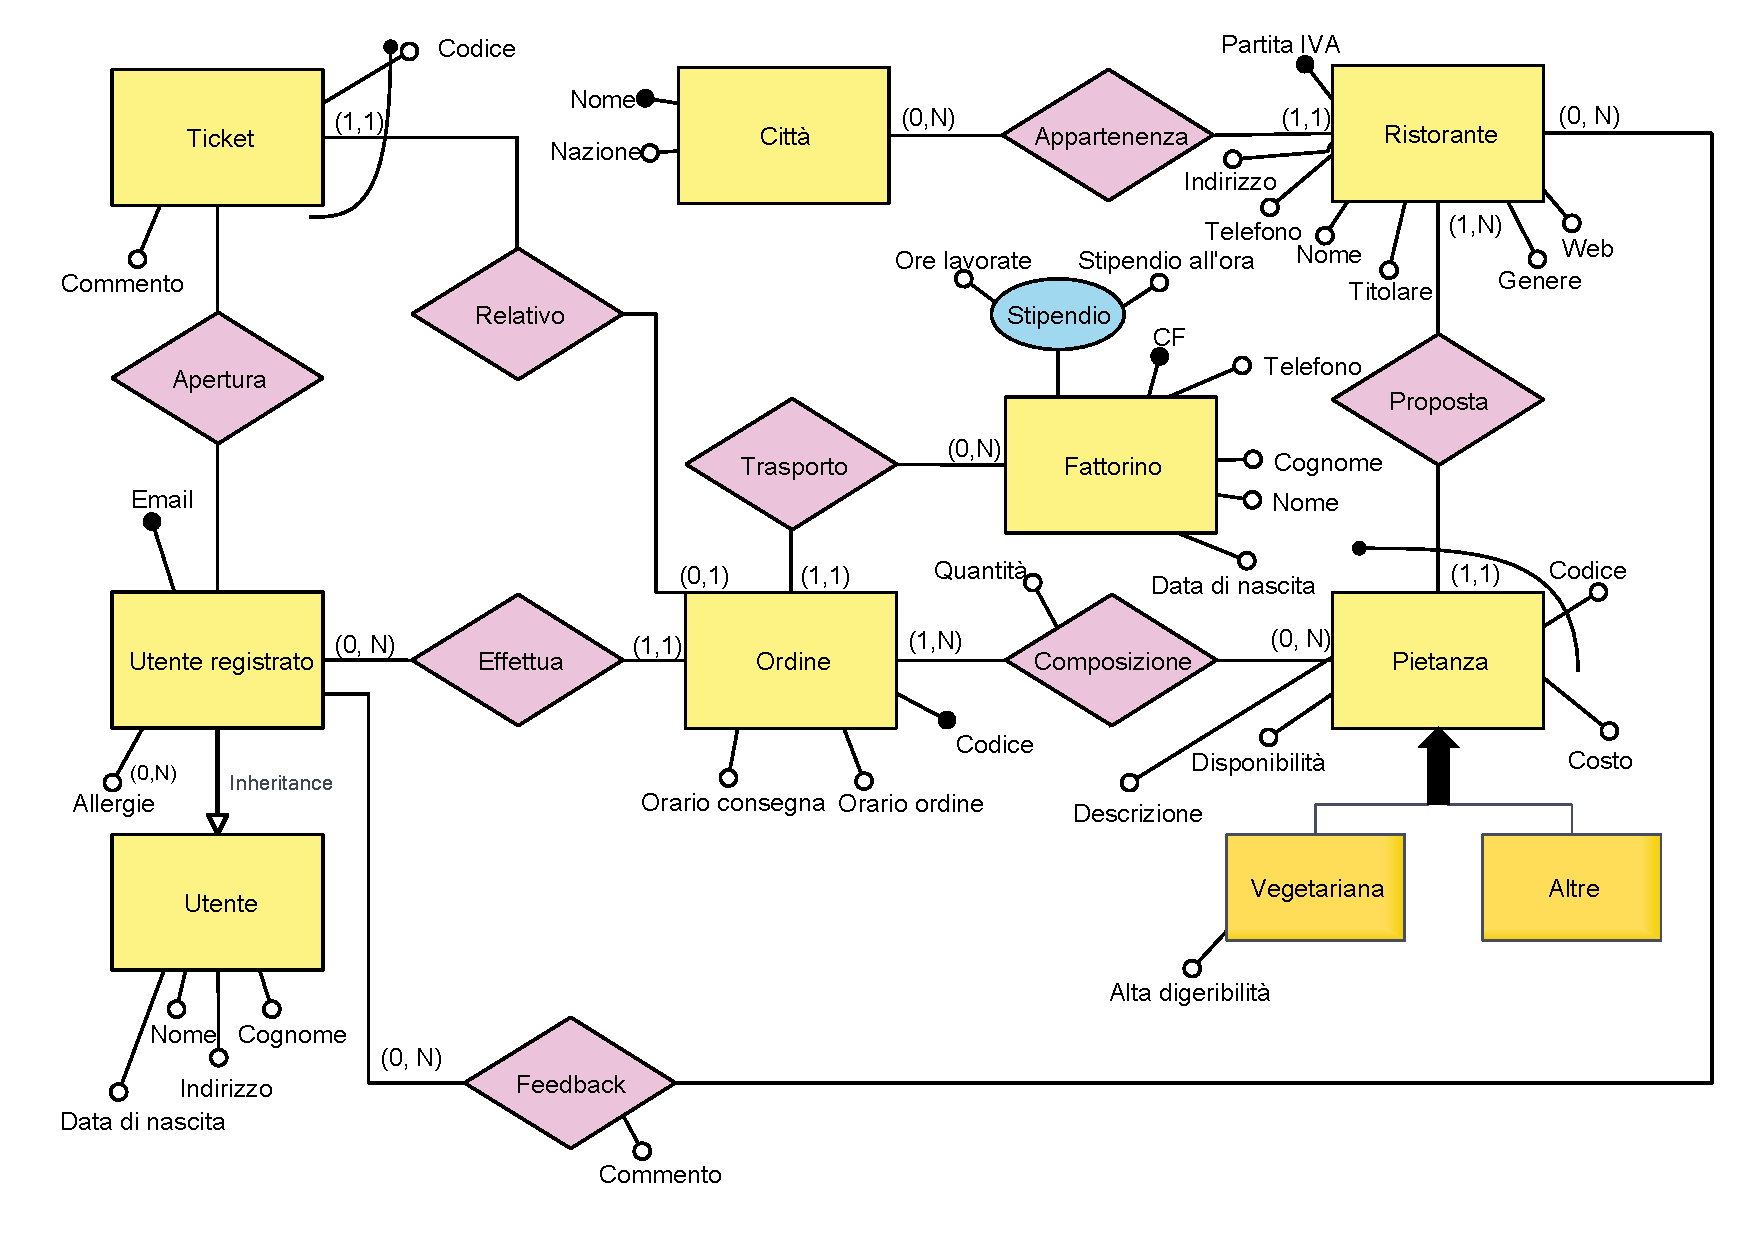
\includegraphics[scale=0.54]{er.pdf}%
				\hspace*{-1cm}%
			\end{center}			
			\caption{Modello ER rappresentativo della base di dati \label{fig:ER1}}
		\end{figure}
	\section{Progettazione logica}
		\subsection{Descrizione testuale dello schema relazionale}
Partendo dallo schema Entit\`a/Relazioni (Figura \ref{fig:ER1}) non ristrutturato possiamo fare alcune osservazioni relativamente alle entit\`a \texttt{Utente} e \texttt{Pietanza}. In particolare, nell'analisi dei requisiti \`e specificato che un utente registrato pu\`o soffrire di una o pi\`u allergie, \`e pertanto necessario trasformare questo attributo \texttt{multivalore} \textit{Allergia} in un'entit\`a indipendente legata tramite una relazione \texttt{molti a molti}. Infatti, ogni utente pu\`o soffrire di una o pi\`u allergie e la stessa allergia potrebbe essere la medesima per pi\`u clienti. Per quanto riguarda l'entit\`a \textit{Pietanza} invece, introduciamo un attributo \texttt{Tipologia} che indica il tipo di pietanza (vegana, composta da carne, ecc), se questa pientanza apparterr\`a alle tipologia vegetariana allora sar\`a necessario conoscere il metodo di cottura della pietanza. Pertanto, la relazione \texttt{Pietanza} avr\`a l'attributo \textit{metodo di cottura} che eventualmente avr\`a valore nullo.  
		\subsection{Ristrutturazione schema E/R}
			\begin{figure}[H]
			\begin{center}
				\hspace*{-1cm}
				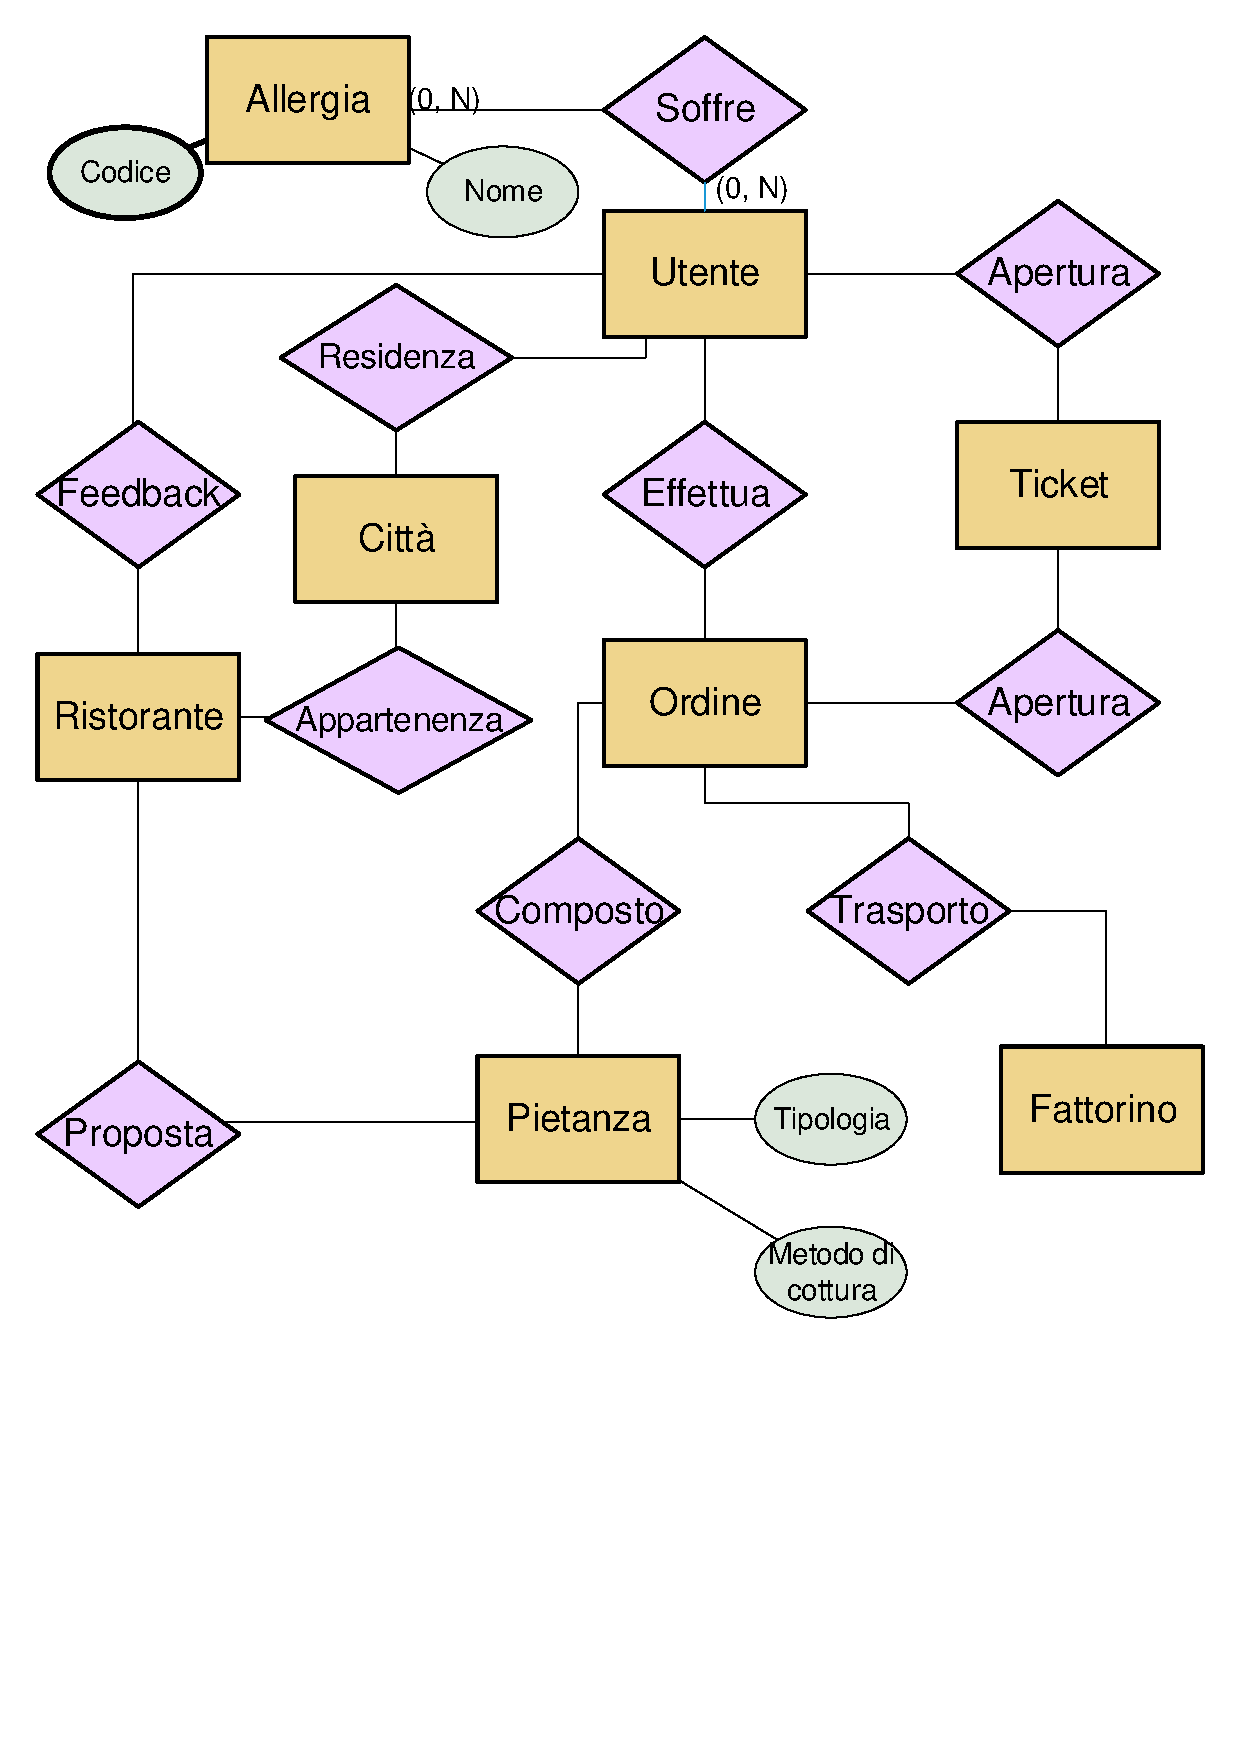
\includegraphics[scale=0.54]{er_ristrutturato.pdf}
				\hspace*{-1cm}
            \caption{Modello E/R ristrutturato, si omettono gli attributi rispetto al modello precedente poich\`e sono gli stessi mentre si introducono le nuove entit\`a }
            \label{fig:ER2}
        	\end{center}
		\end{figure}
			\subsubsection{Cliente} 
			L'attributo multivalore Allergie\footnotemark{} diventer\`a una nuova entit\`a legata a cliente.
			\footnotetext{Le allergie non sono strettamente dipendenti dai clienti.} 
			\paragraph{Attributi aggiornati}
				\begin{itemize}[noitemsep]
						\item Email: \textit{stringa  $\ll$PK$\gg$} - email con la quale il cliente si \`e registrato.
				\end{itemize}
			\subsubsection{Allergia}
				L'entit\`a Allergia conterr\`a il nome dell'allergia e il relativo codice identificativo.
				\paragraph{Attributi}
					\begin{itemize}[noitemsep]
						\item Codice: \textit{intero  $\ll$PK$\gg$} - codice dell'allergia.
						\item Nome: \textit{stringa} - nome dell'allergia.
					\end{itemize}
			\paragraph{Cliente-Allergia: ``Soffre"}
				\paragraph{Molteplicit\`a N:N} Il cliente può soffrire di più allergie, un'allergia può appartenere a più clienti.
				\paragraph{Totalit\`a: parziale verso Allergia/ Totale verso Cliente} Un cliente può non avere allergie, un'allergia appartiene ad almeno un cliente.
			\subsubsection{Pietanza}
			L'entit\`a Pietanza rappresenta l'insieme di pietanze che l'utente può ordinare.
			Rispetto alla precedente entit\`a aggiungiamo gli attributi:
			\begin{itemize}[noitemsep]
				\item Tipologia: \textit{stringa} - tipologia del cibo (i.e. vegana, vegetariana, [...])
				\item Metodo di cottura: \textit{stringa} - indica il metodo di cottura della pietanza.
			\end{itemize}
		\subsection{Schema logico}
			\begin{center}
				\hspace*{-1cm}
				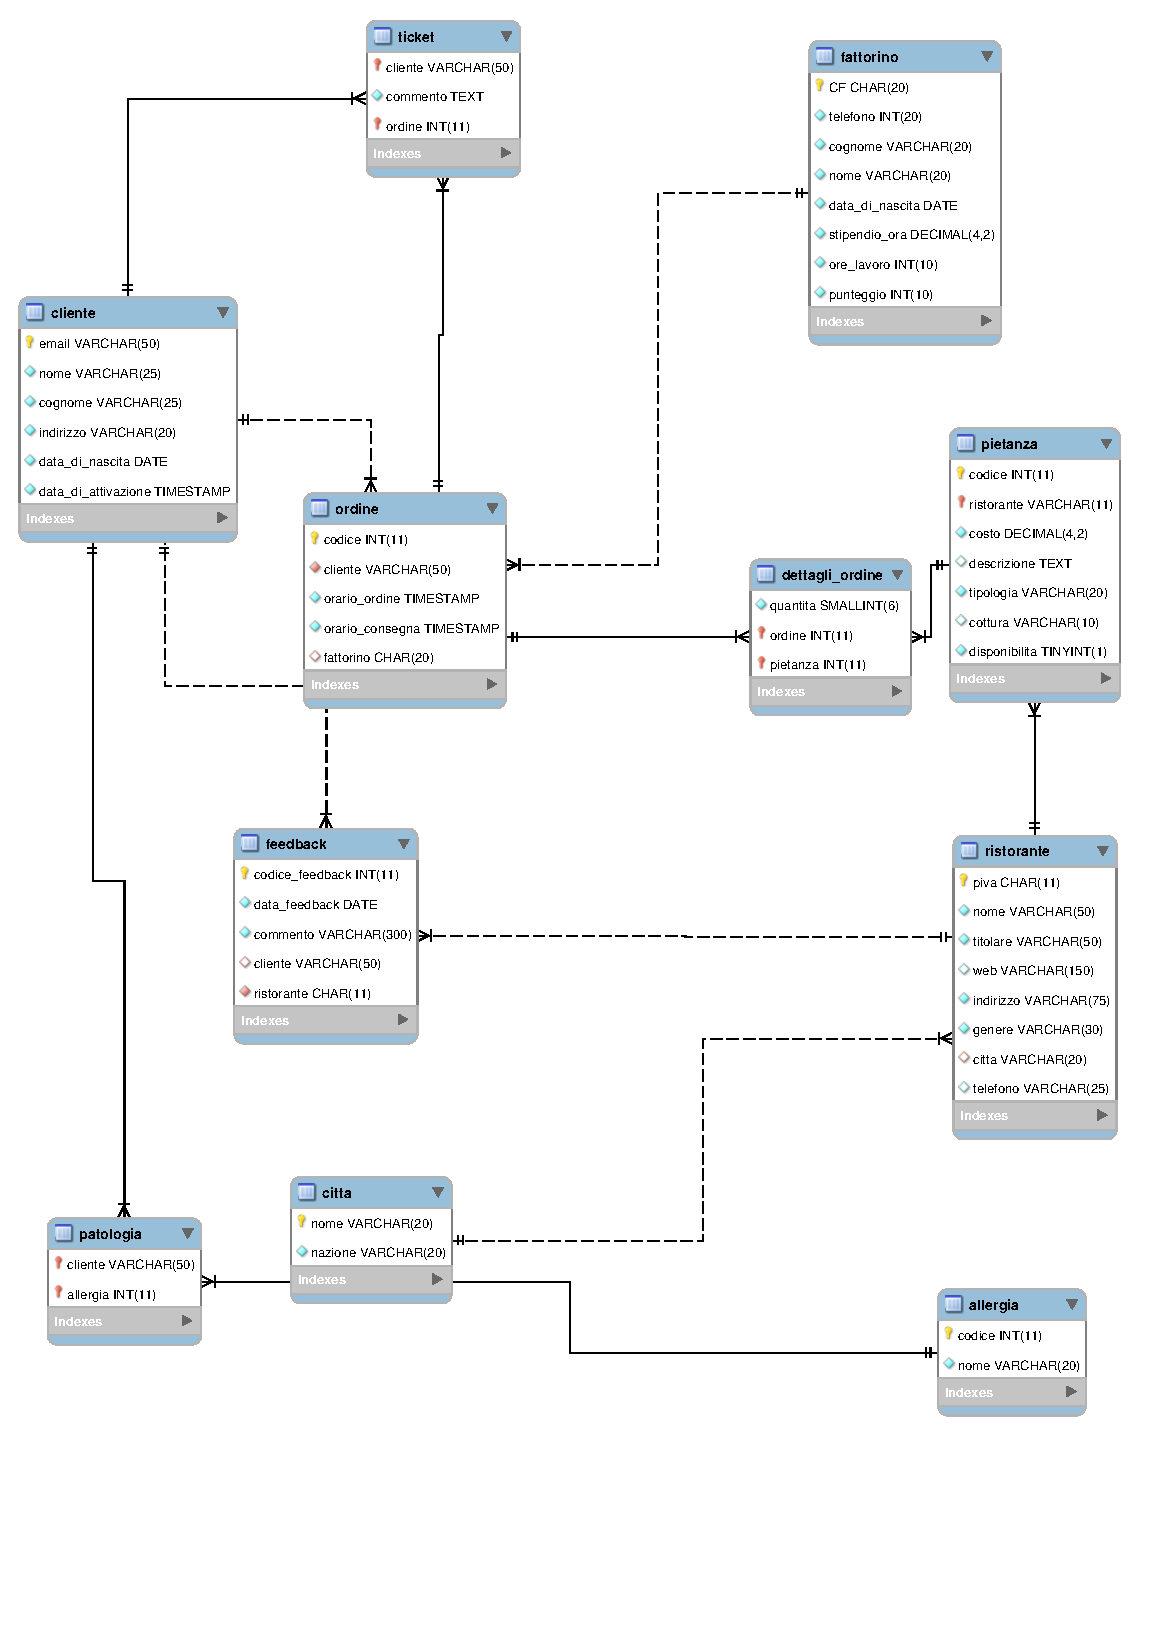
\includegraphics[scale=0.9]{modello_logico.pdf}
				\hspace*{-1cm}
			\end{center}
		\subsection{Modello relazionale}
		\begin{framed}
		\noindent Gli attributi marcati con * sono attrbuti facoltativi che possono avere valore \texttt{\color{blue}NULL}. \newline
		Gli attributi (o l'attributo) \underline{sottolineati/o} indicano una \texttt{CHIAVE}. \newline
		Gli attributi marcati in \textit{corsivo} indicano una \texttt{CHIAVE ESTERNA}.
		\end{framed}
		\begin{itemize}[noitemsep]
			\item[] \textbf{Allergia}(\underline{Codice}, Nome)
			\item[] \textbf{Citt\`a}(\underline{CAP}, Nome, Nazione)
			\item[] \textbf{Cliente}(\underline{Email}, Nome, Cognome, Indirizzo, \textit{Citt\`a}, Data di nascita, Data attivazione account, Allergia\textsuperscript{*})
			\item[] \textbf{Ordine}(\underline{Codice}, Orario ordine, Orario Consegna, \textit{Cliente})
			\item[] \textbf{Ristorante}(\underline{PIVA}, Nome, Titolare, Web, Indirizzo, Telefono, Genere, \textit{Citt\`a})
			\item[] \textbf{Fattorino}(\underline{CF}, Nome, Cognome, Data di nascita, Telefono, Stipendio/h, Ore lavorate)			
			\item[] \textbf{Pietanza}(\underline{Codice}, \underline{\textit{Ristorante}}, Costo, Disponibilit\`a, Descrizione, Tipologia, Metodo di cottura\textsuperscript{*})
			\item[] \textbf{Dettagli Ordine}(\underline{Ordine}, \underline{Pietanza}, Quantit\`a)
			\item[] \textbf{Ticket}(\underline{Codice}, \underline{Ordine}, Commento)
			\item[] \textbf{Feedback}(\underline{Codice}, Cliente, Ristorante, Data commento, Commento)
		\end{itemize}
	\section{Query}
	\begin{enumerate}[noitemsep]
		\item Query che ritorna tutti i codici degli ordini (conclusi e non) e le email dei clienti che li hanno effettuati, nei quali sono stati ordinate solamente pietanze vegetariane cotte a vapore.
\begin{lstlisting}[language=sql]
SELECT o.codice, o.cliente
FROM ordine o JOIN cliente c ON o.cliente = c.email
WHERE NOT EXISTS (
	SELECT *
	FROM ordine o JOIN dettagli_ordine do ON o.codice = do.ordine JOIN pietanza p ON do.pietanza = p.codice
	WHERE cottura <> "VAPORE" AND tipologia <> "VEGETARIANA"
)
\end{lstlisting}
	\item Query che ritorna i codici fiscali di tutti i fattorini che hanno portato a termine tutti gli ordini senza nessun ticket aperto ed hanno ottenuto un punteggio superiore a 10.
\begin{lstlisting}[language=sql]
SELECT cf
FROM (SELECT f.cf, f.punteggio FROM fattorino f
		EXCEPT
	  SELECT f.cf
	  FROM fattorino f JOIN ordine o ON f.cf = o.codice JOIN ticket t ON o.codice = t.ordine)
WHERE punteggio > 10
\end{lstlisting}	
	\end{enumerate}
	\pagebreak
	\section{Eventi, Viste, procedure, trigger e funzioni}
		\subsection{Eventi}
		Nell'analisi dei requisiti viene espressamente richiesto che ogni mese il fattorino pi\`u giovane con punteggio pi\`u alto riceva un incremento stipendiale di 0,20 \euro{} all'ora.
		Le operazioni sulla tabella fattorino vengono delegate alla procedure \texttt{AumentoStip}.
\begin{lstlisting}[language=sql]
DELIMITER $$
	CREATE EVENT MigliorImpiegato
		ON SCHEDULE EVERY '1' MONTH
		STARTS '2018-01-01 00:00:00'
		DO 
		BEGIN
			DECLARE CF_fattorino varchar(20);
			CF_fattorino = SELECT cf FROM fattorino WHERE punteggio = (SELECT MAX(punteggio) FROM fattorino) 
					AND data_di_nascita = (SELECT MAX(data_di_nascita) FROM fattorino);
			CALL AumentoStip(CF_fattorino);
		END$$
DELIMITER ;\end{lstlisting}
		\subsection{Viste}
		\subsection{Procedure}
		\subsection{Trigger}
		Un problema che si viene a creare nella tabella \texttt{Pietanza} con l'impiego di una chiave primaria composta \`e il seguente: Ogni pietanza ha un codice che associato al risorante mi permette di identificare la pientanza. Questo codice per\`o non pu\`o essere settato come \texttt{AUTO\_INCREMENT} perch\`e MySQL non supporta questa funzione con chiavi primarie composte da pi\`u attributi.
		\begin{lstlisting}[language=sql]
DELIMITER $$		
	CREATE TRIGGER `MANUAL_AUTOINCREMENT` BEFORE INSERT ON `pietanza`
		FOR EACH ROW BEGIN
		SET NEW.codice = (
			SELECT MAX(codice) + 1
			FROM pietanza WHERE ristorante = NEW.ristorante
		);
	END $$		
DELIMITER ;\end{lstlisting}
		\subsection{Funzioni}
	\end{document}
